\begin{center}
\bfseries\Large
I-Design: Personalized LLM Interior Designer:\\
Appendix
\end{center}

\section{Additional Qualitative Results}
In this section, we present additional qualitative outcomes. Fig.~\ref{fig:supp:gallery} shows a range of living room renders generated using generic prompts. 
Fig.~\ref{fig:supp:gallery_w_prompt} highlights our method's capability in handling various prompt types. 
Fig.~\ref{fig:supp:scenegraph} illustrates the conversion of a generated scene graph into a 3D representation.


\begin{figure}[H]
  \centering
  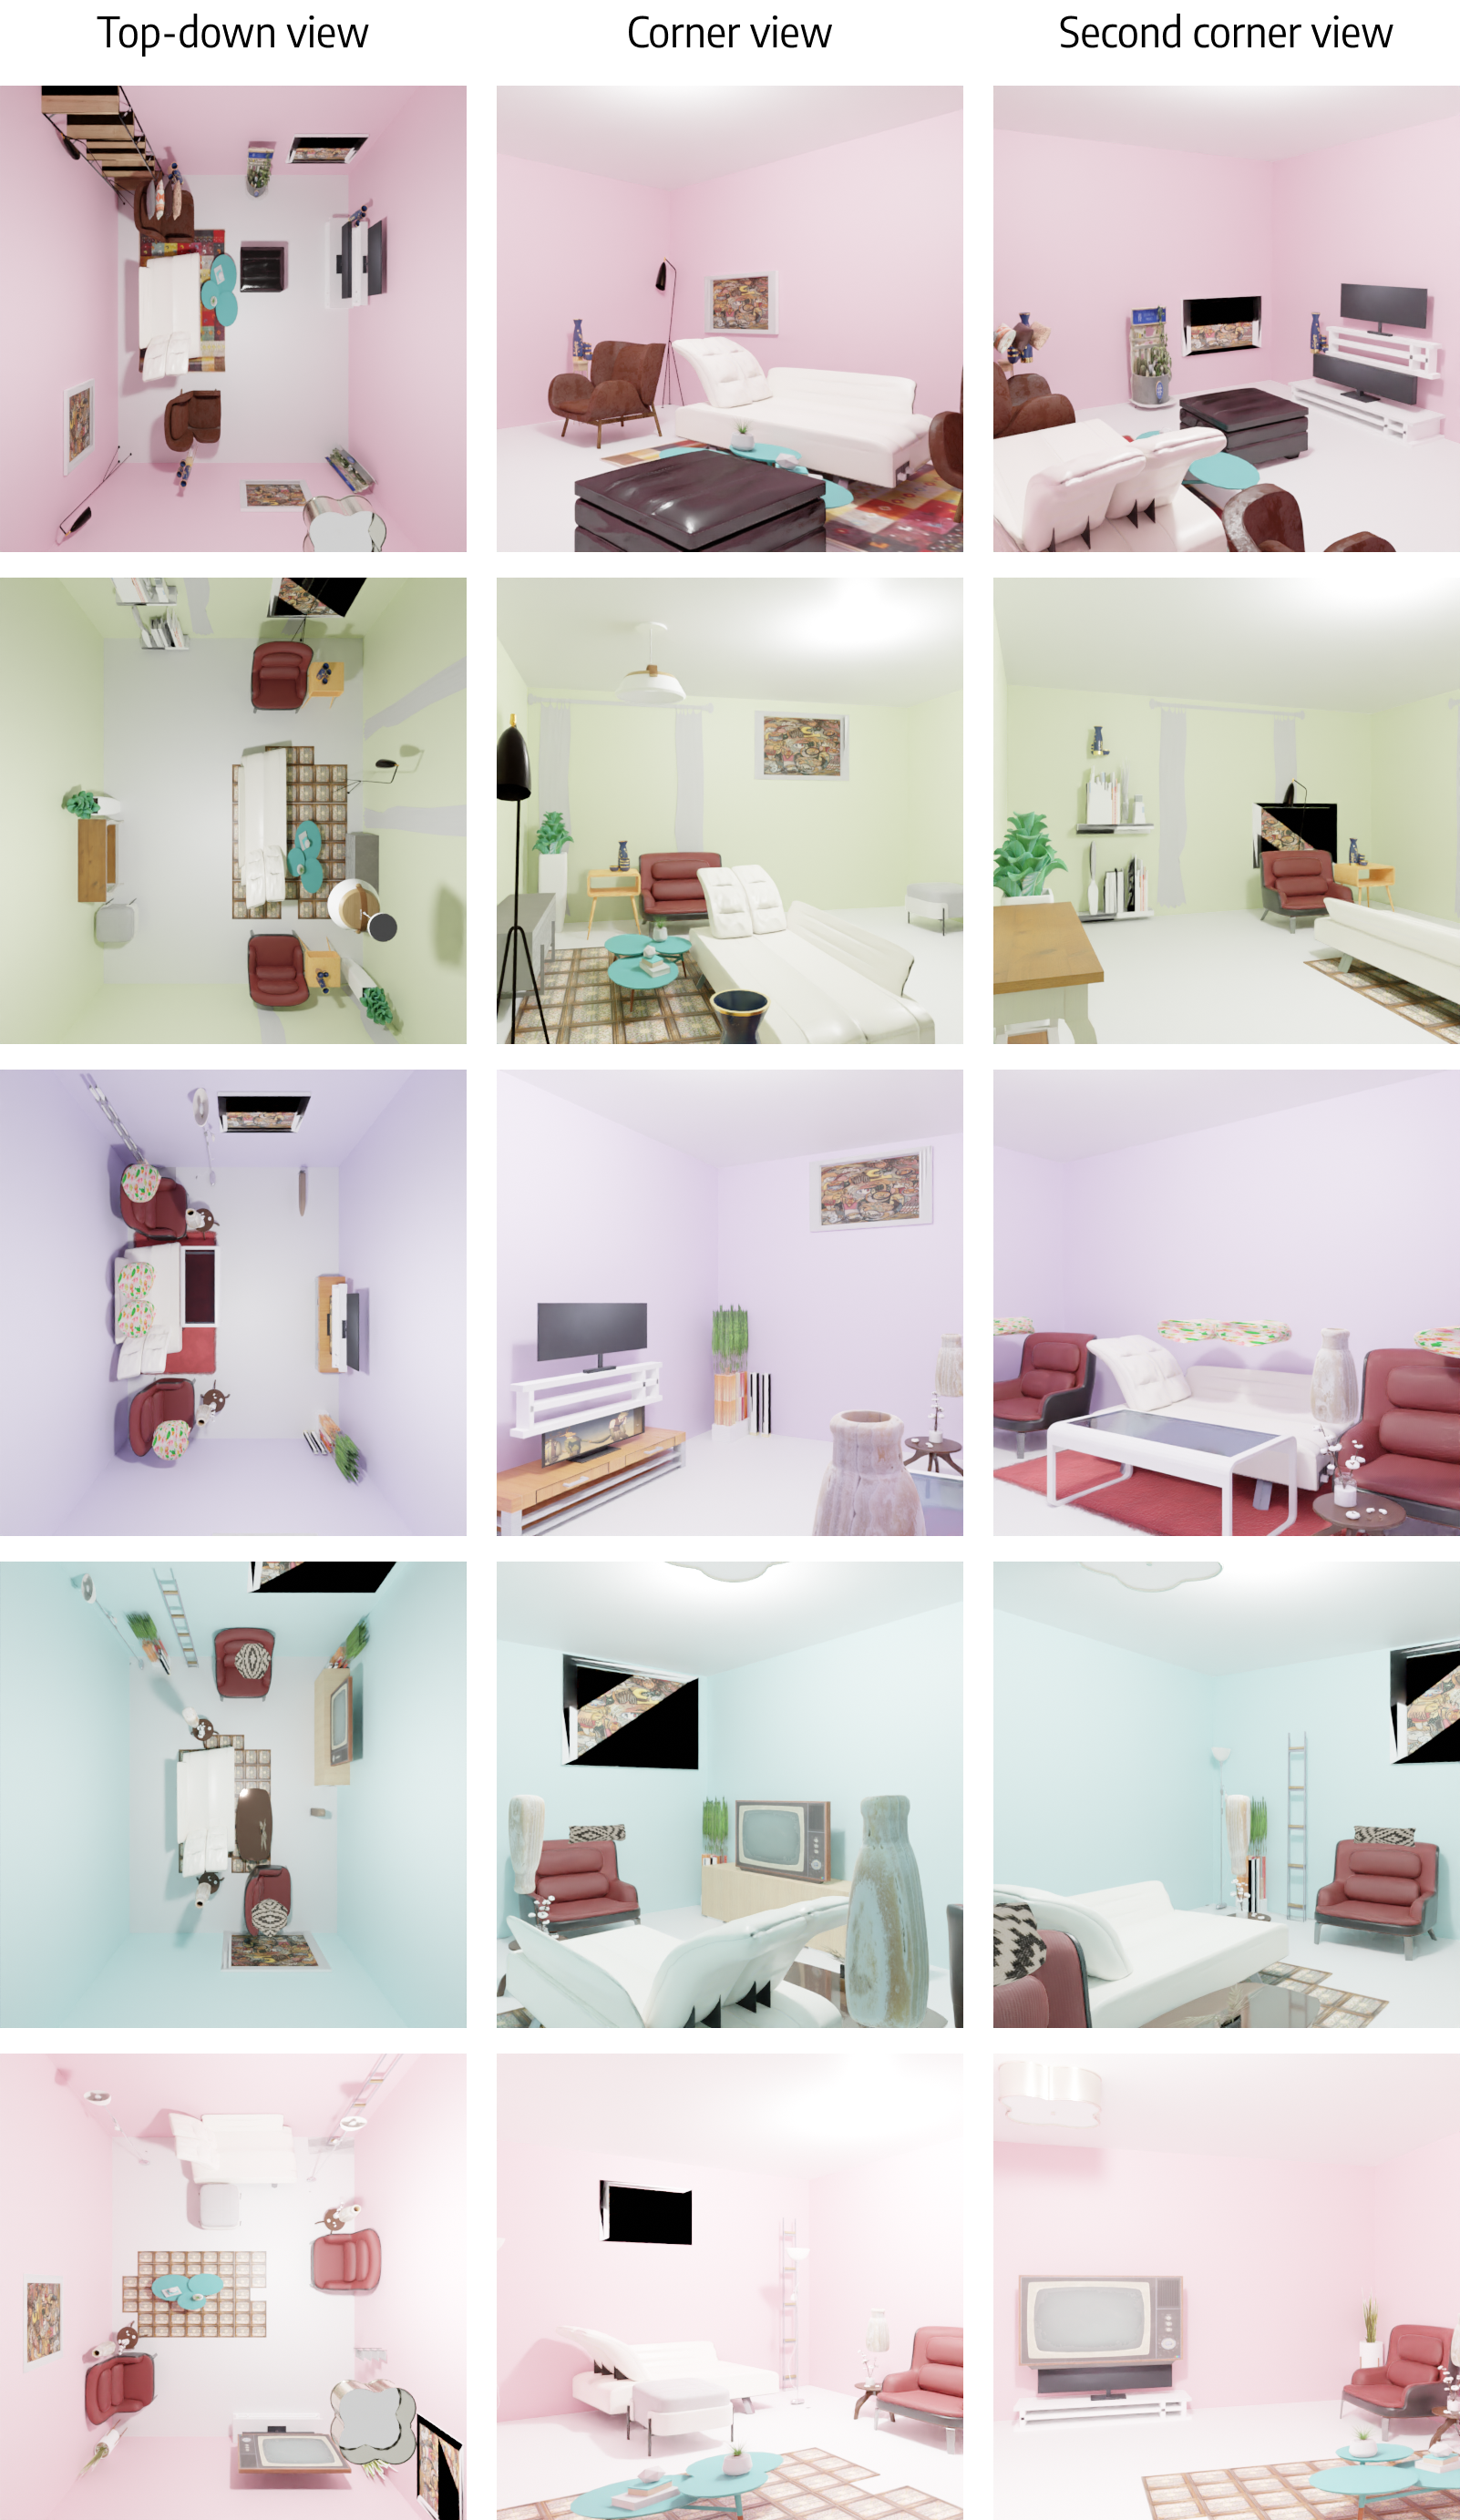
\includegraphics[width=.80\textwidth,clip,trim={0 60em 0 10em}]{images/gallery_supp_liv.png}
  \caption{
    \textbf{Living Room Renders with Generic Prompting.}
    We showcase samples from living room renders used for the comparison with LayoutGPT~\cite{feng2023layoutgpt} in Tab.~\ref{tab:quant_eval} of the main paper. 
    The common prompt for all these scenes is: ``\textit{Design me a living room}''.
  }
  \label{fig:supp:gallery}
\end{figure}

\begin{figure}[H]
  \centering
  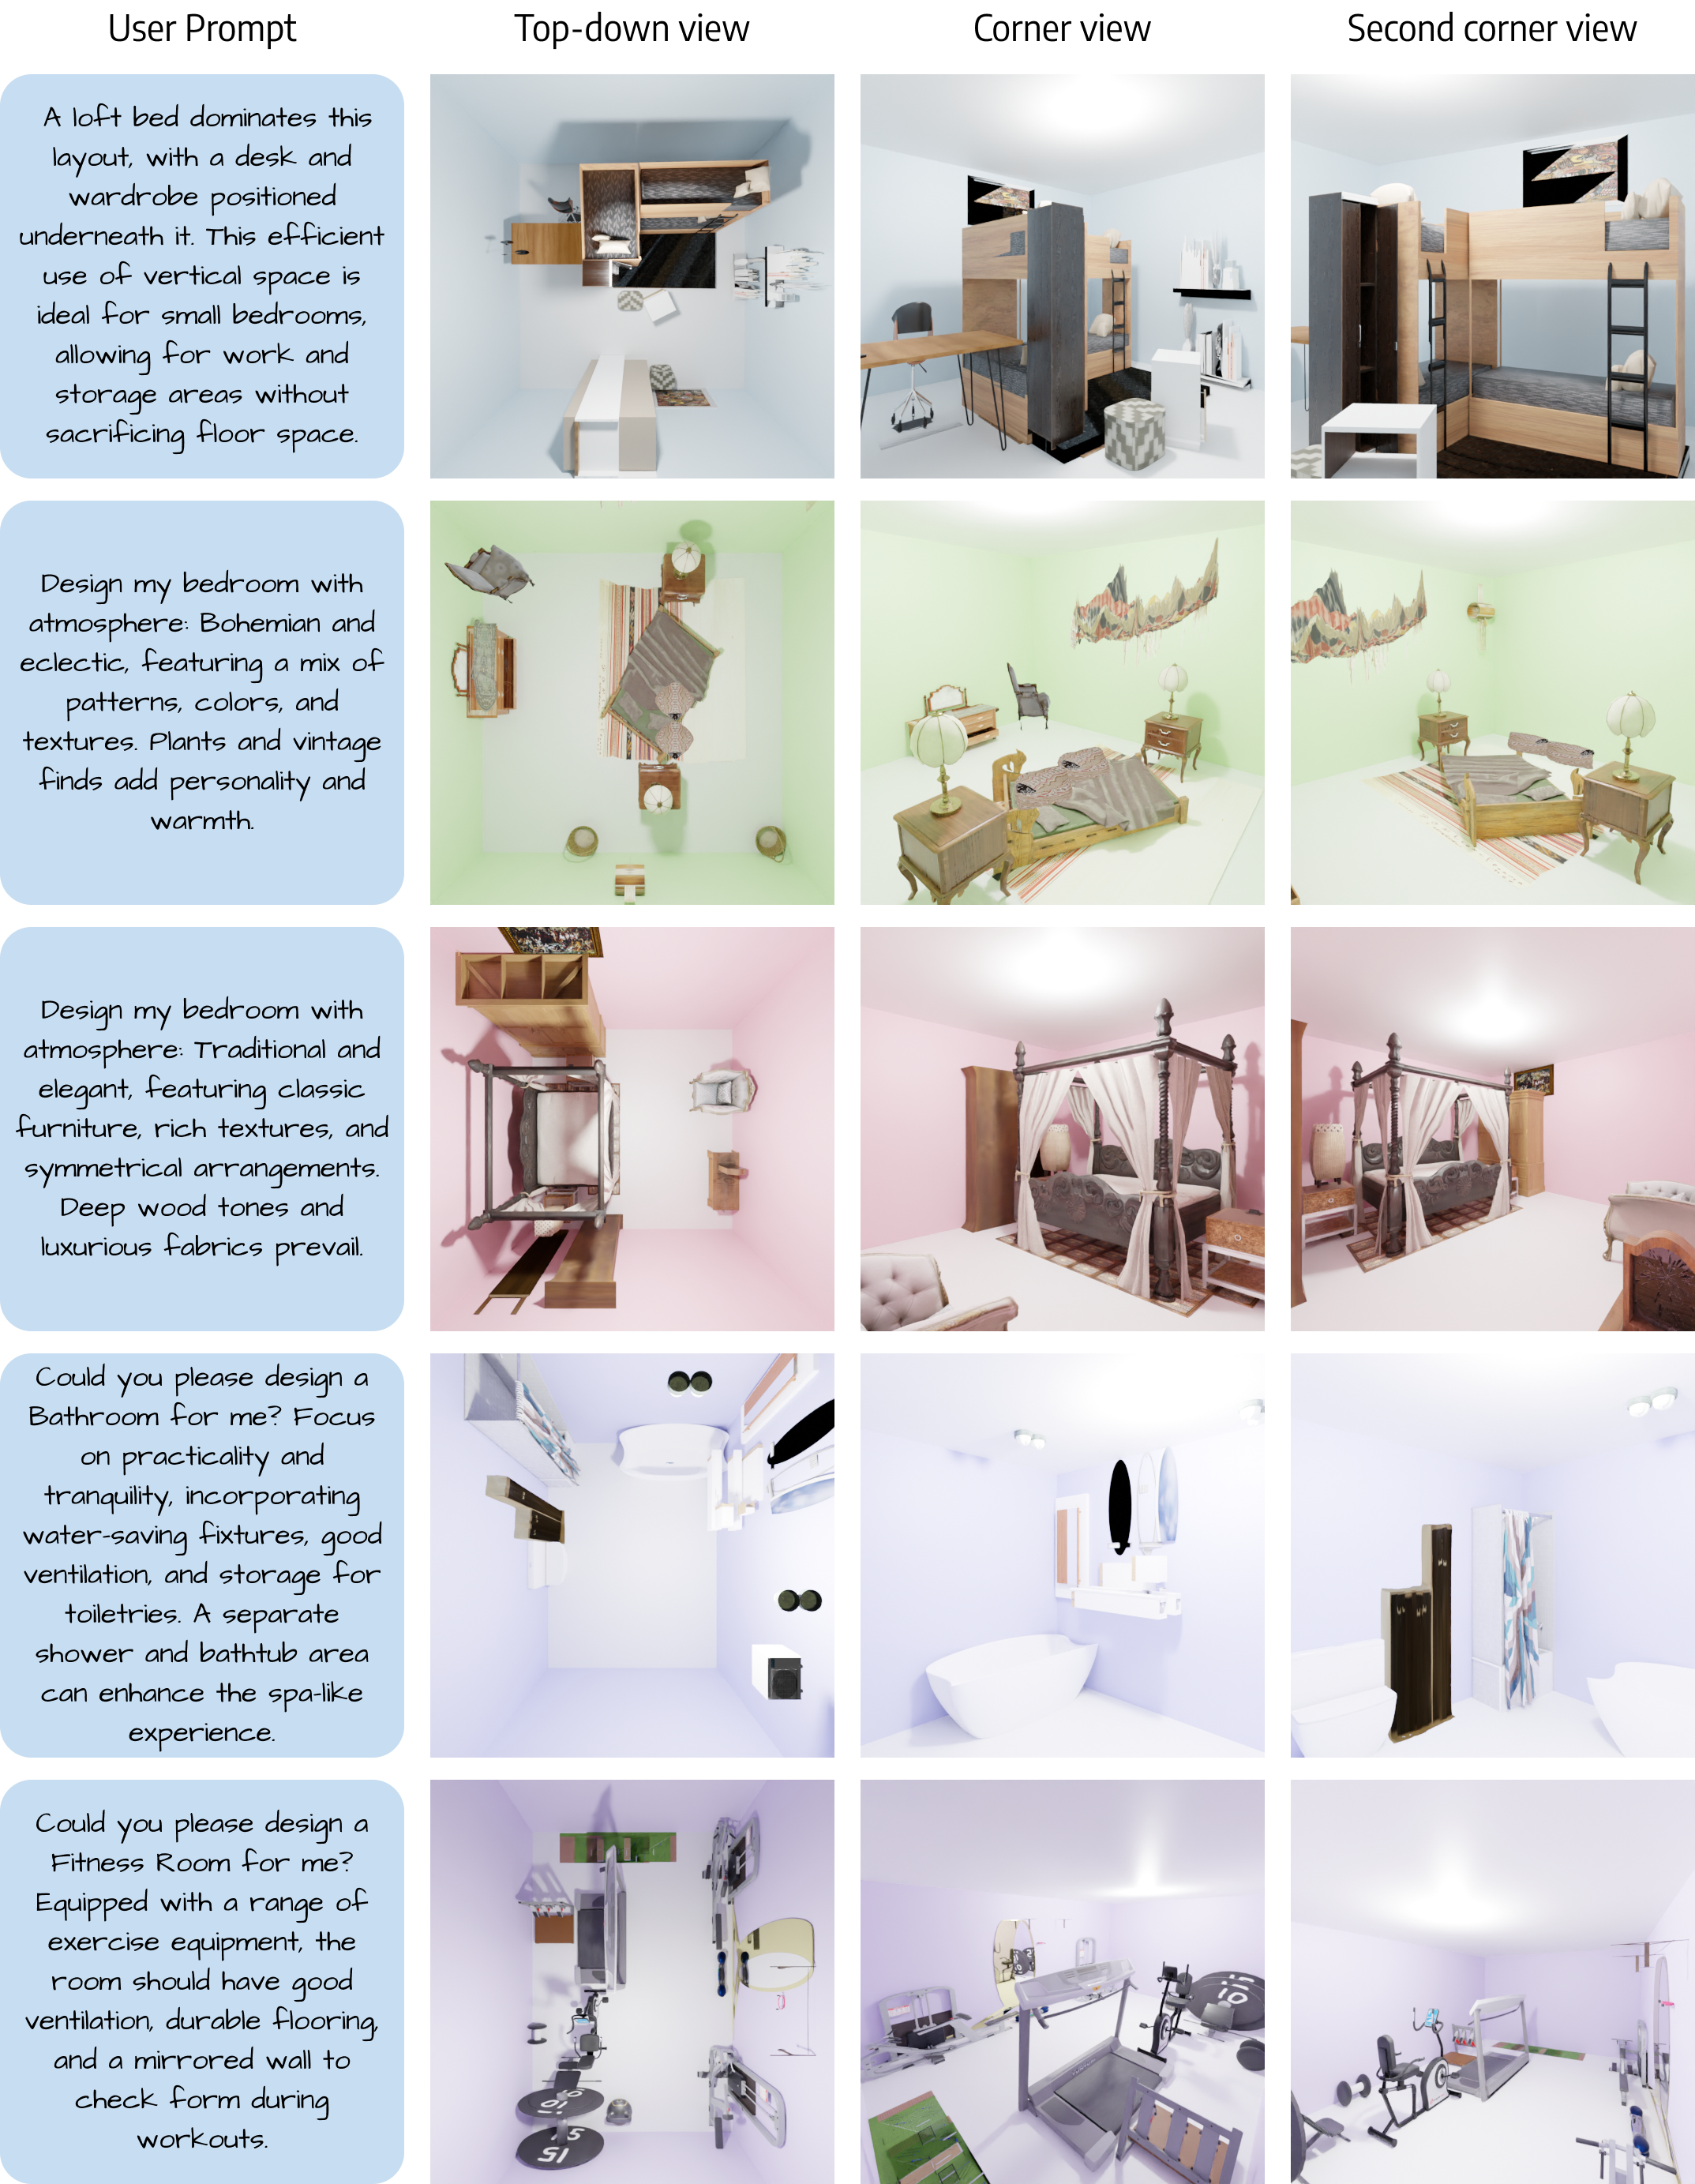
\includegraphics[width=\textwidth,height=\textheight, keepaspectratio]{images/gallery_supp_w_prompt.png}
  \caption{
    \textbf{Generating Renders through Elaborate Prompting}
    This collection presents rendered samples used for the evaluation in Tab.~\ref{tab:prompt_eval_unary} of the main paper. 
    The prompts for generating indoor scenes vary across five categories: Atmosphere, Scheme, Layout, and Functionality.
  }
  \label{fig:supp:gallery_w_prompt}
\end{figure}

\begin{figure}[H]
  \centering
  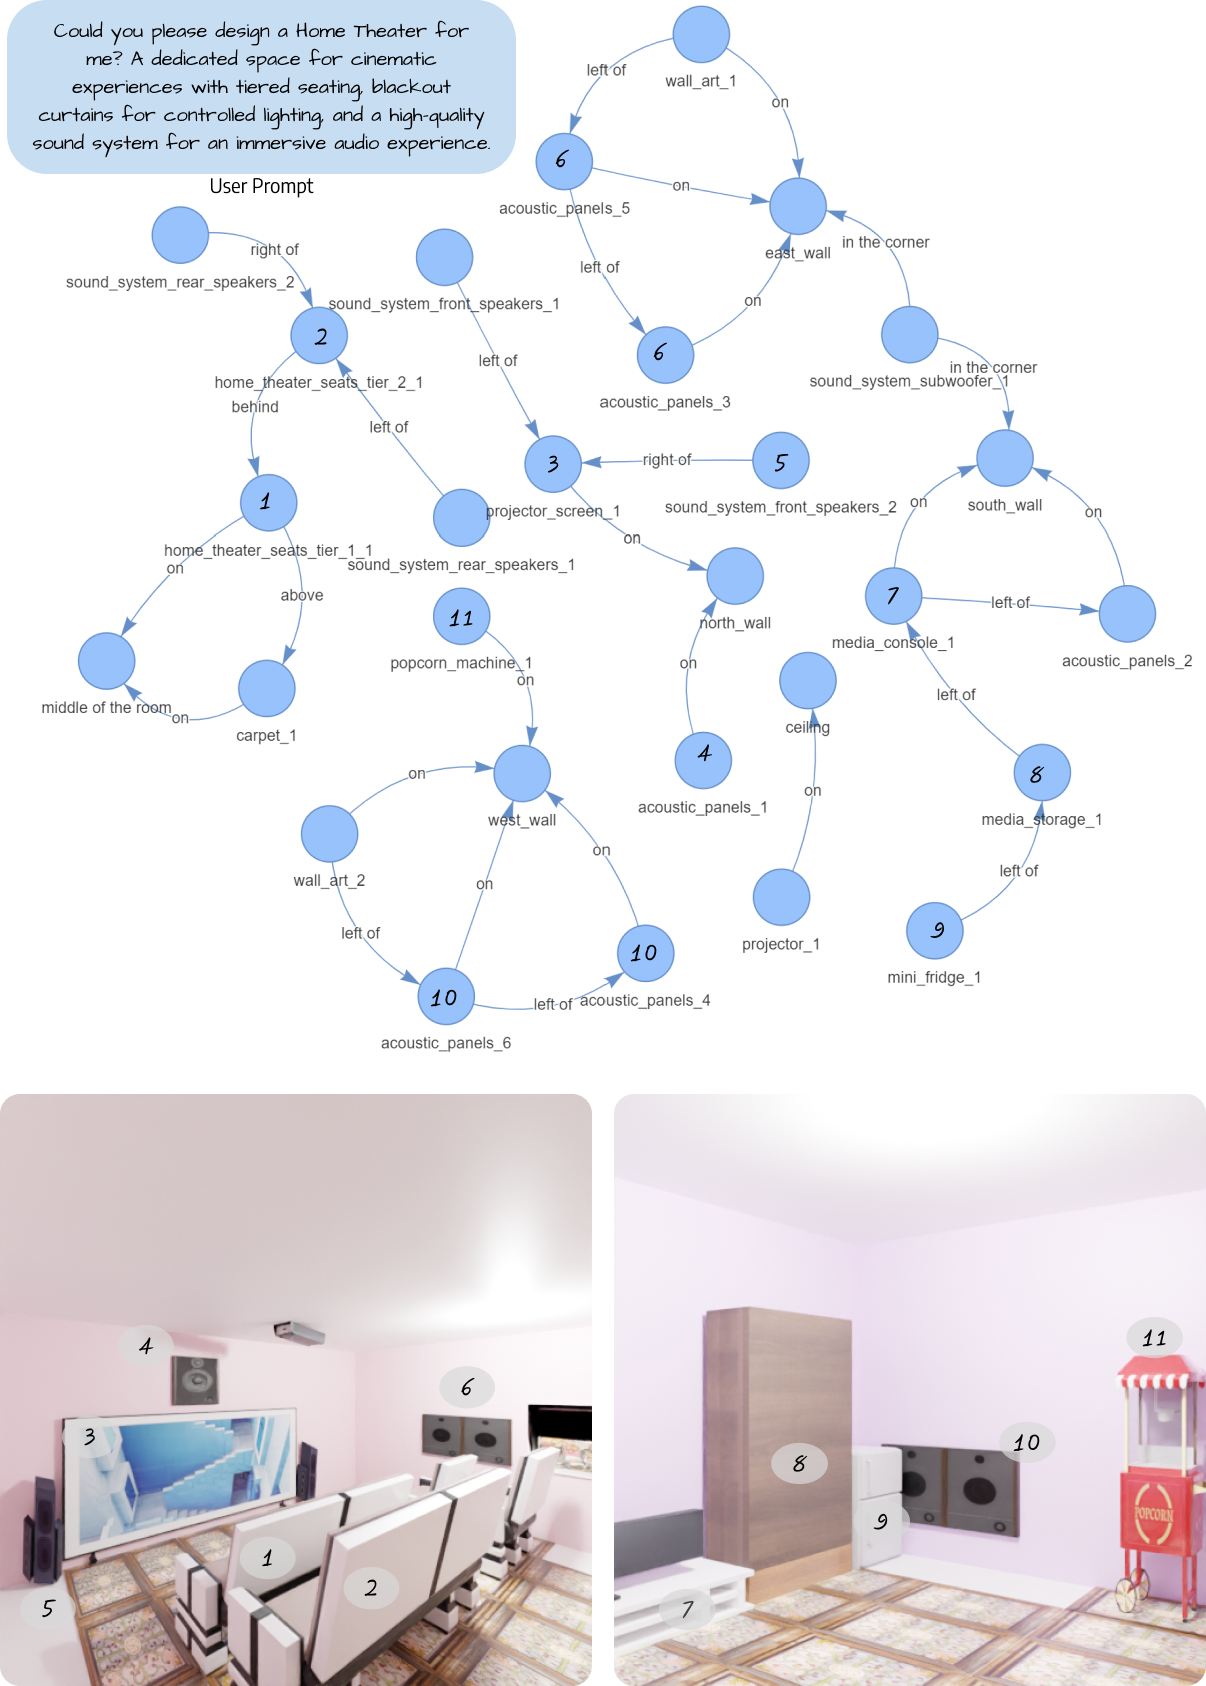
\includegraphics[width=\textwidth,height=\textheight, keepaspectratio]{images/Scene_Graph_Supp_1.png}
  \caption{
    \textbf{Synthesized Scene Graph and Corresponding Renders}
    We illustrate the transformation of a user prompt into a scene graph and then into its corresponding 3D representation.
  }
  \label{fig:supp:scenegraph}
\end{figure}


\section{Implementation of the Multi-agent Pipeline}
As stated in Sec.~\ref{sec:llm-agent}, the responsibility of the Multi-agent pipeline includes suggesting scene objects, determining their relative placements, and structuring this information into a JSON object that conforms to a specified schema. There are a few motivations for distributing these tasks to multiple LLM instances. 

The main reason for following a ``Divide \& Conquer'' approach is the observed performance increase when each LLM instance focuses on solving a more trivial sub-problem by attending to the outputs of the previous agents during communication in an attempt to solve the entirety of the problem iteratively. Adding a feedback loop to the communication process further helps erase unwanted behavior from the agents and tackle hallucination issues.

Additionally, task distribution between agents addresses another challenge: not surpassing the output token limit of the LLM when dealing with a large number of objects. Currently, GPT-4 supports an output token limit of 4000 tokens, which constrains the number of objects and information that an LLM instance can handle in a single iteration. Furthermore, we observed that as LLM outputs approach the token limit, the attention to user and system prompts drastically decreases, resulting in object suggestions or placements that do not align with user preferences. Distributing the information processing among multiple agents mitigates this problem and allows more objects to be successfully generated.

In our implementation, the Interior Designer and Interior Architect agents generate and process all objects together in one pass. This design choice enables the agents to attend to each object effectively. We additionally explored alternative approaches wherein objects would be suggested and placed incrementally as the scene is completed. However, our experiments revealed repetitive object suggestion patterns with these alternative schemes, with some objects repeatedly proposed multiple times. This suggests that as the number of objects in the scene increases, the agents may struggle to comprehend the semi-completed scenes effectively. All GPT-4 agents utilize the ``JSON mode,'' which exclusively restricts their output to the JSON format. This approach further reduces the number of tokens spent in each iteration.

As the Engineer's task solely involves fitting the outputs of the Interior Designer and Architect agents into a specified schema, the Engineer agent can, in contrast, generate structured outputs for each object individually. This step is independent of each object and does not require consideration of other objects in the scene. Due to the aforementioned limitations regarding large output chunks, we opt for an iterative structuring process for the Engineer agent.

\section{Implementation of the GPT-4V Evaluator}
In Sec.~\ref{sec:quantitative}, we presented a grading-oriented evaluation approach leveraging the GPT-4V model. This system enables the measurement and comparison of abstract concepts like atmosphere and color schemes using renders from the scenes. As reflected in Sec.~\ref{sec:user_study}, the findings from the user study align with the GPT-4V evaluation, demonstrating the effectiveness of our LLM-based evaluation method. 

In our current experimental setup, we encode two separate renders of a scene from opposing corners and prompt the GPT-4V evaluator to grade the scene in four categories: Atmosphere, Scheme, Layout, and Functionality. The evaluator is executed three times in total, and the mean grade is calculated to reduce the variability in grades across different runs. 

To stimulate a ``chain of thought'' process~\cite{wei2022chain}, we instructed the GPT-4V evaluator to comment on the scenes regarding various grading aspects before generating the actual grades. This approach enables the model to consider its comments throughout the grading process.

\subsection{GPT-4V Evaluator System Prompt}

Give a grade from 0 to 10 to the following room renders based on how well they correspond together to the user preference (in triple backquotes) in the following aspects:
\\\\
- Realism and 3D Geometric Consistency
\\
- Functionality and Activity-based Alignment
\\
- Layout and furniture  
\\
- Color Scheme and Material Choices
\\
- Overall Aesthetic and Atmosphere   
\\\\
User Preference:
``\textbf{\{prompt\}}''
\\\\
Return the results in the following JSON format:
``\textbf{\{example\_json\}}''

\section{Discussion}

In this section, we delve into the existing limitations of our pipeline and potential future research directions.

One limitation stems from the LLM's inability to consider multiple factors simultaneously (including the rotation of the parent object, placement of other children, availability of space, and so forth) when integrating an object into a scene, particularly as the scene becomes more complex.
Thus, as the scene graph grows, the likelihood of the LLM suggesting unreasonable relational edges among objects increases. Likewise, as the number of objects in the scene increases, LLMs struggle to monitor the remaining available space, which may result in an overflow of objects in certain parts of the scene.


Another issue arises due to the discrepancy between the bounding box scale ratios inferred by the LLM and the actual asset retrieved. A laptop is a good example of such a case since closed and open laptops have very different bounding box ratios. If the agent infers a closed laptop, but the retrieved asset is an open laptop, the renders may result in visually implausible outcomes with distortions because of the resizing process. A similar discrepancy might also arise for object orientations. The canonical orientation of an asset might differ from the canonical orientation inferred by agents. For example, determining the front side of a desk can be subjective. The front side might be considered where a person would typically place a chair, or it could be perceived as the opposite side.

To maintain a consistent and immersive atmosphere, cohesive texture becomes essential. However, the original textures of retrieved objects from the dataset cannot be guaranteed to align seamlessly with user preference. Achieving precise control over texture and geometry-related features remains challenging despite extracting assets from large-scale datasets guided by text embeddings to ensure semantic alignment. Future work may consider incorporating a re-texturing step to enhance the coherence of the overall atmosphere. 

Lastly, we place objects in the scene with a bounding box assumption, meaning that the objects are assumed to have quadratic surfaces. While this approach simplifies the spatial representation of 3D objects and prevents collisions, it can lead to spatial inconsistencies when placing child objects, especially when placing a child object on top of a parent object. This limitation may result in artifacts such as ``floating'' objects. For further work, we encourage exploring an extra step that utilizes mesh surfaces instead of bounding boxes for precise placement.      

\section{System Prompts for Agents}

Creating the scene graph involves various agents, each playing a distinct role within the overall generation process. These roles are imparted to the agents through ``system prompts,'' shaping their responses to user prompts and instilling them with individual characteristics. These prompts help define each agent's functionality and guide them in generating structured outputs. The system prompts for each agent are provided verbatim below. The JSON schemas provided to each agent (highlighted with \textbf{\{json\_schema\}}) are included in the supplementary files and the project webpage.

\subsection{Interior Agent System Prompt}

Interior Designer. Suggest \{n\} essential new objects to be added to the room based on the user preference, the general functionality of the room, and the room size. The suggested objects should contain the following information:
\\\\
1. Object name (ex., bed, desk, chair, monitor, bookshelf, etc.)
\\\\
2. Architecture style (ex., modern, classic, etc.)
\\\\
3. Material (ex., wood, metal, etc.)
\\\\
4. Bounding box size in meters (ex., Length: 1.0m, Width: 1.0m, Height: 1.0m). Only use ``Length'', ``Width'', and ``Height'' as keys for the bounding box size.
\\\\
5. Quantity (ex., 1, 2, 3, etc.)
IMPORTANT: Do not suggest any objects related to doors or windows, such as curtains, blinds, etc.
\\\\
Follow the JSON schema below:
\textbf{\{json\_schema\}}

\subsection{Interior Architect System Prompt}
Interior Architect. Your role is to analyze user preferences, consider the optimal placement for each object that the Interior Designer suggests, find a place for this object in the room, and give a detailed description of it.
If the quantity of an object is greater than one, you have to find a place for each instance of this object separately but give all this information in one list item.
Give explicit answers for EACH object on the following three aspects:
\\\\
Placement: 
Find a relative place for the object (e.g., in the middle of the floor, in the northwest corner, on the east wall, right of the desk, on the bookshelf).
For relative placement with other objects in the room, use the prepositions ``on'', ``left of'', ``right of'', ``in front'', ``behind'', ``under''.
For relative placement with the room layout elements (walls, the middle of the room, ceiling), use the prepositions ``on'' and ``in the corner''.
You are not allowed to use any prepositions other than the ones above. Explicitly state the placement for each instance (ex., one is on the left of desk\_1, one is on the south\_wall).
\\\\
Proximity : 
Proximity of this object to the relative placement objects:
\\
1. Adjacent: The object is physically contacting the other object, or the other object supports it, or they are touching, or they are close to each other.
\\
2. Not Adjacent: The object is not physically contacting the other object and is distant from it.
\\\\
Facing :
Think about which wall (west/east/north/south\_wall) this object should be facing and explicitly state this (ex., one is facing the south\_wall, one is facing the west\_wall).
\\\\
If the quantity of an object is greater than one, you have to find a place for each instance of this object separately but give all this information in one list item.
\\\\
Follow the JSON schema below:
\textbf{\{json\_schema\}}

\subsection{Engineer System Prompt}
Engineer. You listen to the input by the Admin and create a JSON file.
\\\\
When the Admin outputs objects to be in the room, you will save ALL of them in the given schema.
For the scene graph, you can use the IDs for the objects already in the room but only output the objects to be placed.
If an object has a quantity higher than one, save each instance of this object separately.
\\\\
IMPORTANT: The inputted ``Placement'' key should be used for the ``placement'' key in the JSON object. Follow exactly the prepositions stated; do not use the information in the ``Facing'' key for the room layout elements.
\\\\
IMPORTANT: For object quantities greater than one, the ``placement'' key gives separately the relative placement of each instance of that object in the room; make the distinction for each instance accordingly.
\\\\
Use only the following JSON Schema to save the JSON object:
\textbf{\{json\_schema\}}

\subsection{Layout Corrector System Prompt}
Layout Corrector Agent. Whenever a user provides an object that doesn't fit the room for various spatial conflicts, you will change its ``scene\_graph'' and ``facing\_object'' keys to resolve these conflicts. 
\\\\
You will use the JSON Schema to validate the user's JSON object.
\\\\
For relative placement with other objects in the room, use the prepositions ``on'', ``left of'', ``right of'', ``in front'', ``behind'', ``under''.
For relative placement with the room layout elements (walls, the middle of the room, ceiling), use the prepositions ``on'', and ``in the corner''.
\\\\
Use only the following JSON Schema to save the JSON object:
\textbf{\{json\_schema\}}

\subsection{Layout Refiner System Prompt}
Layout Refiner. Whenever the Admin speaks, you will look at the parent object and children objects, the first preposition that connects these objects, and find a second suitable relative placement for the children objects while considering the initial positioning of the object. 
Give the relative placement of the children objects with each other and with the parent object. For example, if there are five children objects ``on'' the parent object, give the relative positions of the children objects to one another and the second preposition to the parent object (``on'' is the first preposition).
\\\\
Use only the following JSON Schema to save the JSON object:
\textbf{\{json\_schema\}}

\section{Room Synthesis Prompt Generation for Evaluation}
Our proposed pipeline aims to serve as a personalized interior design assistant capable of offering tailored design suggestions based on diverse user inputs, reflecting various preferences and requirements. Our motivation is to construct prompts that reflect the authentic comments real people might make when designing their rooms. 

In the realm of interior design, the significance of both aesthetics and functionality is consistently emphasized~\cite{ching2018interior}. A deeper exploration of personalized interior design, as articulated in~\cite{lee2022conceptual}, identifies four pivotal aspects central to decision-making: indoor space components, human tendencies, technology, and spatial evaluation. Indoor space components encompass factors such as materials, layout, and arrangement, while human tendencies consider individual inclinations influenced by past experiences and personalities. Spatial evaluation accentuates productivity, underlining the importance of creating environments conducive to efficient work.

Drawing from this framework, we establish our GPT-4V evaluation criterion and generate prompts by varying key elements, including functionality, layout, color scheme with material choice, and overall atmosphere. These prompts are generated utilizing GPT-4. For instance, in generating prompts related to functionality, we instruct GPT-4 to provide descriptions for different room types, incorporating varied functionalities and dimension specifications. Similarly, for prompts assessing layout, color scheme, and overall atmosphere alignment, we maintain fixed room types and dimensions while altering layout, color scheme, or atmosphere. We generate ten prompts for each alignment consideration. Below are the prompts for generating room preferences and a comprehensive list of prompts used in the evaluations~\cref{tab:quant_eval} and \cref{tab:prompt_eval_unary} of the main paper.

\subsection{Prompts for Room Preferences Text Generation} 
In the evaluation recorded in \cref{tab:quant_eval}, we utilize minimal preference descriptions as prompts for room synthesis. The prompt for generating these preferences is noted in the section titled ``Minimal Preference Generation Prompt'' below. The preferences generated for room synthesis evaluation in \cref{tab:prompt_eval_unary} of the main paper are listed in the other sections.
\\\\
\noindent
\textit{\textbf{Minimal Preference Generation Prompt}} \\
\textit{Bedroom: }\\
You are a helpful assistant.\\
Could you please provide a list of common dimensions for a bedroom? Please list ten potential dimensions, including width, length, and height in meters. Format your response as follows: [[width, length, height], [width, length, height], ...]
\\\\
\textit{Livingroom: }\\
You are a helpful assistant. \\
Could you please provide a list of common dimensions for a living room? Please list ten potential dimensions, including width, length, and height in meters. Format your response as follows: [[width, length, height], [width, length, height], ...]
\\\\
\noindent
\textit{\textbf{Functionality-related Preference Generation Prompt}}\\
You are a helpful assistant who is designed to output JSON. \\
Please provide ten interior design instructions emphasizing functionality. \\
Begin by specifying the room type and desired room dimensions in meters, including width, length, and height. Describe the room's intended functionality succinctly. Besides, common suggestions also extend to more diverse requirements, such as creating a reading corner or a movie area. \\
Keep descriptions brief, within three sentences, and exclude details involving windows and doors. Aim for diversity in interior room types.\\
Provide the results in JSON format: \{``room type'': \{``dimension'': [width, length, height], ``functionality'': ``functionality description''\}, ``room type'': \{``dimension'': [width, length, height], ``functionality'': ``functionality description''\}, ...\} Note: you need to replace the key ``room type'' with specified room type, such as bedroom, living room etc. 
\\\\
\noindent
\textit{\textbf{Layout-related Preference Generation Prompt}}\\
You are a helpful assistant designed to output JSON.\\
Could you outline ten descriptions of potential bedroom interior design layouts? Please do not include descriptions about style, theme, etc, and only focus on layout.\\
Please present the results in JSON format as follows: \{``1'': ``layout and furniture description'', ``2'': ``layout and furniture description'', ...\}. Please keep each description concise with two to three sentences.
\\\\
\noindent
\textit{\textbf{Color-scheme-and-material-related Preference Generation Prompt}}\\
You are a helpful assistant designed to output JSON.\\
Can you list ten interior bedroom design requirements or ideas with different color themes (e.g., room with pink color colors or beige tones) and material emphasis (e.g., room with wooden elements or metallic elements)? Please do not use windows, ceilings, floors, and walls in the descriptions. \\
Provide the results in JSON format: \{``1'': ``requirement description'', ``2'': ``requirement description'', ...\}. Please keep the description short, with no more than four sentences.
\\\\
\noindent
\textit{\textbf{Overall-atmosphere-related Preference Generation Prompt}}\\
You are a helpful assistant designed to output JSON.\\
Can you provide ten concise descriptions of the overall atmosphere for potential bedroom interior designs? \\
Please present the results in JSON format as follows: \{``1'': ``atmosphere description'', ``2'': ``atmosphere description'', ...\}. Please keep each description concise within two to three sentences.

\subsection{Complete Lists of Prompts}
The comprehensive prompts list for room synthesis evaluations documented in \cref{tab:quant_eval} of the main paper is provided in Tab.~\ref{tab:promtlist_minimal} below. Similarly, the prompts for evaluations recorded in \cref{tab:prompt_eval_unary} are detailed in Tab.~\ref{tab:promtlist_others}.

\begin{longtable}{
    >{\arraybackslash}p{2cm} 
    >{\arraybackslash}p{6cm} 
    >{\centering\arraybackslash}p{4cm}
}
\caption{\textbf{Complete List of Prompts for Evaluation Recorded in \cref{tab:quant_eval} of the main paper.} Prompts 1 to 10 describe \textit{bedrooms};  11 to 20 describe \textit{living rooms}.} \\
\label{tab:promtlist_minimal} \\
\toprule
\textbf{Index} & \textbf{Prompt} & \textbf{Room Dimension} \\
\midrule
\endfirsthead
\multicolumn{3}{c}{{\bfseries \tablename\ \thetable{} -- Continued from previous page}} \\
\toprule
\textbf{Index} & \textbf{Prompt} & \textbf{Room Dimension} \\
\midrule
\endhead
\bottomrule
\multicolumn{3}{c}{{\bfseries Continued on next page}}
\endfoot
\bottomrule
\endlastfoot
1 & Design me a bedroom. & [3.0, 4.0, 2.4] \\
2 & Design me a bedroom. & [2.5, 3.0, 2.4] \\
3 & Design me a bedroom. & [3.5, 4.5, 2.4] \\
4 & Design me a bedroom. & [4.0, 5.0, 2.4] \\
5 & Design me a bedroom. & [2.4, 3.5, 2.4] \\
6 & Design me a bedroom. & [3.2, 4.2, 2.4] \\
7 & Design me a bedroom. & [2.8, 3.6, 2.4] \\
8 & Design me a bedroom. & [3.6, 4.8, 2.4] \\
9 & Design me a bedroom. & [4.2, 5.2, 2.4] \\
10 & Design me a bedroom. & [3.0, 3.5, 2.4] \\
11 & Design me a living room. & [4.0, 5.0, 2.8] \\
12 & Design me a living room. & [3.5, 4.5, 2.8] \\
13 & Design me a living room. & [3.0, 4.0, 2.8] \\
14 & Design me a living room. & [4.5, 6.0, 3.0] \\
15 & Design me a living room. & [5.0, 7.0, 3.0] \\
16 & Design me a living room. & [3.6, 4.8, 2.8] \\
17 & Design me a living room. & [4.2, 5.2, 2.8] \\
18 & Design me a living room. & [5.5, 6.5, 3.0] \\
19 & Design me a living room. & [3.2, 4.2, 2.8] \\
20 & Design me a living room. & [6.0, 8.0, 3.0] 

\end{longtable}

\begin{longtable}{
    >{\arraybackslash}p{1.2cm} 
    >{\arraybackslash}p{8cm} 
    >{\centering\arraybackslash}p{2.5cm}
}
\caption{\textbf{Complete List of Prompts for Evaluation Recorded in \cref{tab:prompt_eval_unary} of the main paper.} Prompts from index 1 to 10 pertain to \textit{functionality} preferences, those from index 11 to 20 concern \textit{layout}, index 21 to 30 relate to \textit{color scheme and materials}, and prompts from index 31 to 40 encompass \textit{overall atmosphere} preferences.} \\
\label{tab:promtlist_others} \\
\toprule
\textbf{Index} & \textbf{Prompt} & \textbf{Room Dimension} \\
\midrule
\endfirsthead
\multicolumn{3}{c}{{\bfseries \tablename\ \thetable{} -- Continued from previous page}} \\
\toprule
\textbf{Index} & \textbf{Prompt} & \textbf{Room Dimension} \\
\midrule
\endhead
\bottomrule
\multicolumn{3}{c}{{\bfseries Continued on next page}}
\endfoot
\bottomrule
\endlastfoot
1 & Could you please design a Living Room for me? Designed for relaxation and socializing, the living room should feature comfortable seating areas, ample lighting for different activities, and a designated movie area with a large screen and surround sound for an immersive experience. & [6, 8, 2.5] \\
2 & Could you please design a Home Office for me? The home office should prioritize a clutter-free workspace with ergonomic furniture, ample storage for office supplies, and a small area for breaks with a comfortable chair and a coffee machine. & [3, 4, 2.5] \\
3 & Could you please design a Kitchen for me? Efficiency and ease of movement are key, with a triangular layout between the stove, refrigerator, and sink. Include a central island for additional workspace and seating for casual dining. & [5, 7, 2.5] \\
4 & Could you please design a Bedroom for me? A cozy and restful environment with a comfortable bed, soft lighting, and ample storage for personal items. A small reading nook with a comfy chair and a bookshelf should be included. & [4, 5, 2.5] \\
5 & Could you please design a Bathroom for me? Focus on practicality and tranquility, incorporating water-saving fixtures, good ventilation, and storage for toiletries. A separate shower and bathtub area can enhance the spa-like experience. & [3, 4, 2.5] \\
6 & Could you please design a Dining Room for me? Designed for meal gatherings, it should have a large table with comfortable seating for the family and guests, along with ambient lighting to enhance the dining experience. & [4, 6, 2.5] \\
7 & Could you please design a Playroom for me? A vibrant and flexible space that encourages play, creativity, and learning, with durable, easy-to-clean surfaces, storage for toys, and a comfortable area for reading and crafts. & [4, 6, 2.5] \\
8 & Could you please design a Fitness Room for me? Equipped with a range of exercise equipment, the room should have good ventilation, durable flooring, and a mirrored wall to check form during workouts. & [4, 6, 2.5] \\
9 & Could you please design a Laundry Room for me? A functional space with efficient appliances, a fold-out ironing board, and storage for cleaning supplies to make laundry tasks easier and organized. & [3, 3, 2.5] \\
10 & Could you please design a Home Theater for me? A dedicated space for cinematic experiences with tiered seating, blackout curtains for controlled lighting, and a high-quality sound system for an immersive audio experience. & [5, 7, 2.5] \\
11 & Design my bedroom with following layout: This layout features a queen-sized bed against the main wall, with two nightstands on either side. Opposite the bed, there's a dresser with a mirror above it, creating a functional dressing area. & [4, 4, 2.5] \\
12 & Design my bedroom with following layout: In this setup, a single bed is placed in the corner, maximized for space efficiency. A small desk and chair fit snugly in the opposite corner, with a tall bookshelf beside it, making it ideal for a student. & [4, 4, 2.5] \\       
13 & Design my bedroom with following layout: This layout utilizes a king-sized bed centered on the main wall, with a bench at its foot. A large wardrobe is placed on the adjacent wall, providing ample storage space without cluttering the room. & [4, 4, 2.5] \\
14 & Design my bedroom with following layout: A twin bed is positioned against one wall, leaving space for a play area on the opposite side of the room. Toy storage and a small table with chairs are included in the play area, perfect for children. & [4, 4, 2.5] \\
15 & Design my bedroom with following layout: The room features a full bed flanked by a desk on one side and a nightstand on the other. Across from the bed, a low media console serves as a place for entertainment equipment, optimizing the layout for relaxation and study. & [4, 4, 2.5] \\
16 & Design my bedroom with following layout: In this compact layout, a murphy bed is installed to maximize floor space when not in use. A fold-down desk is mounted on the opposite wall, creating a multipurpose space that can easily transition from bedroom to home office. & [4, 4, 2.5] \\
17 & Design my bedroom with following layout: A loft bed dominates this layout, with a desk and wardrobe positioned underneath it. This efficient use of vertical space is ideal for small bedrooms, allowing for work and storage areas without sacrificing floor space. & [4, 4, 2.5] \\
18 & Design my bedroom with following layout: This spacious layout includes a queen-sized bed positioned centrally with a vanity table and stool set against the adjacent wall. A comfortable reading chair and floor lamp are placed in one corner, creating a cozy reading nook. & [4, 4, 2.5] \\
19 & Design my bedroom with following layout: Featuring a platform bed with storage drawers beneath, this layout optimizes storage. Along the opposite wall, a long, low dresser doubles as a display surface for personal items, with a mirror above it to enhance natural light. & [4, 4, 2.5] \\
20 & Design my bedroom with following layout: In this innovative layout, the bed is centrally located with a headboard that doubles as a room divider. Behind the headboard, a workspace is created with a desk and shelving, effectively separating the sleeping and working areas. & [4, 4, 2.5] \\
21 & Design a bedroom with color theme Minimalist with White Tones for me. Use white and light grey hues to emphasize cleanliness and simplicity. Incorporate sleek, modern furniture with straight lines. Material focus on matte finishes and textiles like cotton or linen for a soft touch. & [4, 4, 2.5] \\
22 & Design a bedroom with color theme Boho Chic with Earthy Tones for me. Focus on mixing patterns, colors, and textures. Use materials like rattan, bamboo, and unfinished woods. Incorporate plants and macrame textiles for a cozy, natural feel. & [4, 4, 2.5] \\
23 & Design a bedroom with color theme Industrial with Metallic Elements for me. Incorporate exposed steel, iron, or brushed nickel finishes in decor items and furniture. Use a neutral palette with bold accents in art or textiles. Emphasize raw and unfinished looks. & [4, 4, 2.5] \\
24 & Design a bedroom with color theme Modern Glam with Gold Accents for me. Use a base of neutral colors with pops of bold color. Integrate gold-trimmed furniture and gold accent decor for a touch of luxury. Velvet and silk fabrics add texture and opulence. & [4, 4, 2.5] \\ 
25 & Design a bedroom with color theme Nautical with Blue Colors for me. Incorporate various shades of blue with crisp white for a sea-inspired look. Use striped patterns and nautical decor items. Materials include weathered wood and rope accents for a maritime feel. & [4, 4, 2.5] \\
26 & Design a bedroom with color theme Scandinavian with Pastel Colors for me. Use pale blues, pinks, and greens on a backdrop of white or grey. Furniture is minimalist and functional, with natural light wood materials. Add cozy textiles like wool or mohair to enhance comfort. & [4, 4, 2.5] \\
27 & Design a bedroom with color theme Rustic with Wooden Elements for me. Emphasize natural, unfinished woods in furniture and decor for a warm, earthy feel. Use leathers and woven textiles to add depth. Incorporate organic, handmade items to underscore the rustic theme. & [4, 4, 2.5] \\
28 & Design a bedroom with color theme Art Deco with Rich Jewel Tones for me. Combine deep greens, blues, and purples with metallic accents in gold or brass. Use geometric patterns in textiles and art. Furniture and decor pieces should evoke the luxury and opulence of the 1920s and 1930s. & [4, 4, 2.5] \\
29 & Design a bedroom with color theme Contemporary with Monochromatic Scheme for me. Stick to a monochromatic color scheme throughout, using varying shades of the same color for depth. Focus on sleek furniture with minimalist designs. Utilize textures like glass, polished metals, and smooth fabrics to add interest. & [4, 4, 2.5] \\
30 & Design a bedroom with color theme Vintage with Floral Patterns for me. Incorporate floral patterns in textiles, art, and wallpaper. Use a mix of antique or vintage-style furniture with rich wood tones. Embrace lace and embroidered textiles for a delicate, classic touch. & [4, 4, 2.5] \\
31 & Design my bedroom with atmosphere: Minimalist and serene, with clean lines and a monochrome palette. Accentuated by natural light and a lack of clutter. & [4, 4, 2.5] \\
32 & Design my bedroom with atmosphere: Bohemian and eclectic, featuring a mix of patterns, colors, and textures. Plants and vintage finds add personality and warmth. & [4, 4, 2.5] \\
33 & Design my bedroom with atmosphere: Modern and sleek, characterized by bold geometric shapes and a neutral color scheme. Innovative lighting and high-tech elements are key. & [4, 4, 2.5] \\
34 & Design my bedroom with atmosphere: Cozy and rustic, emphasizing natural wood, stone, and warm, earthy tones. Chunky knits and a fireplace complete the inviting ambiance. & [4, 4, 2.5] \\
35 & Design my bedroom with atmosphere: Nautical and breezy, with a color palette of blues, whites, and sandy tones. Maritime accessories and striped patterns evoke the seaside. & [4, 4, 2.5] \\
36 & Design my bedroom with atmosphere: Glamorous and luxurious, marked by opulent fabrics, metallic finishes, and a touch of sparkle. Elegant furniture and plush textiles dominate. & [4, 4, 2.5] \\
37 & Design my bedroom with atmosphere: Industrial and edgy, with exposed brick, metal details, and raw concrete elements. A neutral color scheme is offset by vibrant art. & [4, 4, 2.5] \\
38 & Design my bedroom with atmosphere: Traditional and elegant, featuring classic furniture, rich textures, and symmetrical arrangements. Deep wood tones and luxurious fabrics prevail. & [4, 4, 2.5] \\
39 & Design my bedroom with atmosphere: Scandinavian and bright, with a focus on simplicity, functionality, and minimalism. Pale woods, muted colors, and hygge accents are key. & [4, 4, 2.5] \\
40 & Design my bedroom with atmosphere: Contemporary and dynamic, with a mix of textures and materials. Clean lines, pops of color, and versatile pieces adapt to changing trends. & [4, 4, 2.5] 

\end{longtable}
